\chapter{Table Recognition Implementation}

This chapter gives us an overview of procedures and tools used to create a table recognition software. 

The implementation is divided into two main parts --- \emph{preprocessing}, which consists of parsing arguments from command line and image manipulation, and \emph{tabular OCR}, which calls a character recognition software and given the output data, determines the presence of tables in the input images.

\section{Preprocessing}

The preprocessing part of the implementation is mostly only an interface representing everything that could still be implemented. It consists of two parts --- a parser and a preprocessor.

\emph{The parser} is used for processing the input command line arguments. It also contains a configuration class, which saves the values of preprocessing arguments and filenames that need to be processed. This is later used in the preprocesser. 

The main function of the parser is a function of the configuration class \emph{parse\_args()}. It takes all of the command line arguments and initializes the configuration class with the given values. If no value has been specified, the current preprocessing option will not be implemented. The only exception to this is the command line option \emph{-p} of \emph{--preprocess}, which initializes the preprocessing option values to those that had the best results overall.

The \emph{parse\_args()} function also parses the filenames and directory names of the files that will be processed. The parser therefore also contains functions for file manipulation, like creating directories, subdirectories, determination of files or directories, extracting the filename from path and other. 

After the parsing part is done, processing of the individual images begins. This is done in a for loop for each file returned from the parser. Images are therefore processed one by one.

Although we need only one copy of the image for passing to the preprocessor and then processing, we keep another copy during the whole run of the program. Therefore, once the recognition algorithm is over, the result can be displayed on the original image to prevent the user from seeing the output of the preprocessor, as the preprocessed image may be too noisy, hard to read and will most likely lose most of the color information.

First step of the processing is the call of the \emph{preprocessor}, concretely its \emph{preprocess\_file()} function that proceeds by calling the individual preprocessing functions depending on the configuration settings. In this implementation, only the basic preprocessing options are available, e.g. enhancing, deskewing, greyscale conversion and binarization. These are all implemented in the Leptonica library which also provides the calls of these functions. 

The initial idea for preprocessing was to provide more complex functions which are included in the OpenCV library. However, this was not the goal of the thesis. Therefore, the preprocessing part stayed very simple and mostly demonstrative and the user is still advised to preprocess the images manually.

However, preprocessing is a crucial part when it comes to OCR. We will discuss its importance and the options of improvement (like usage of OpenCV, determination of the need to preprocess etc.) in the next sections \xxx{pridat odkazy}. 

\section{Tabular OCR}

The actual table recognition is executed in a \emph{process} file along with a \emph{utils} file that contains a few helper functions. The main function called is a function of a page class, \emph{process\_image()}, that executes our table detection algorithm.

This is also the place where the already mentioned Tesseract engine is integrated and called. In our algorithm, as well as the Tesseract table detection algorithm, we use the already implemented Tesseract line and symbol detection. Therefore, our algorithm relies greatly on the functioning of the Tesseract engine. 


\subsubsection{Algorithm implementation}

Our algorithm is based on the already mentioned Tesseract symbol and textline recognition and moreover on whitespace detection. Upon detecting whitespaces between individual symbols, we try to heuristically estimate the whitespaces between words and, furthermore, columns, for each textline of the image. Once we have all the textlines separated into columns, we try to merge consecutive lines with similar columns into a table.  

In this section, we will analyze this algorithm step-by-step and overview the functions used.

\begin{description}
\item[Textline initialization] The whole process begins with initialization of individual textlines. This is the only place where we use the character recognition from the Tesseract software.

We initialize the Tesseract API without the use of neural networks and obtain both lines and symbols from the API. Then, we iterate over all the lines and symbols and try to assign symbols into lines to which we think they might belong to. The result of this function is therefore a list of all textlines that contain the information about their individual symbols, like positioning and their actual value in UTF8.

This function runs in $O(m*n^2)$. The initial idea for this implementation was to firstly sort both the symbols and lines by their y coordinates (which is simply $O(\log n)$ and  $O(\log m)$) and iterate the cycle in $O(m*n)$ by simply iterating symbols and jumping to another line once symbol does not fit in the given line. This would mean a significant improvement in the time complexity. However, a problem occurred when iterating symbols. By default, Tesseract recognizes anything it can find and assumes it to be a symbol. This creates a lot of false positives, including noise recognized as dots, white spaces, and, most importantly, horizontal or vertical lines, like footer or header separators, underlinings of words, table borders etc. We tried to adjust our algorithm to ignore empty characters. Horizontal and vertical line detection, however, was a harder task. Although most of the lines are pretty simple to detect (either their width or height is significantly greater than the other, or either width or height is unusually small in comparison to other characters), there is no one criterion that would suffice all lines, with problems occurring mostly at thick but short lines. Therefore, we sacrificed \xxx{dobre slovo?} the time complexity in favor of accuracy.

This function is the place where most of the mistakes are made and time complexity is consumed. Although a robust software, Tesseract recognition is still far from ideal and sometimes fails at even the simplest images. Also, its recognition takes up significantly more time than all of the other functions combined. We will discuss the details of Tesseract recognition complexity and errors and their possible improvements in following chapters.

\item[Deletion of unnecessary lines]

As already mentioned, Tesseract recognition algorithm includes a lot of false positives. In this function, we delete all unnecessary lines, specifically:

\begin{itemize}
\item\textbf {Empty lines: } Like horizontal or vertical line segments, borders or other lines that contain no UTF8 symbols are of no use and are therefore deleted from the textline list.

\item\textbf {Table textlines: } Table textlines are parts of the image that already had a border around them, which might have been either a table, form or even a graphics image. Tesseract often recognizes these parts as single textlines. These textlines therefore contain multiple other textlines, and are significantly greater in height. We delete these textlines by simply looking at their height and the font of their symbols.
\end{itemize}

\begin{figure}[H]
\begin{subfigure}{0.45\textwidth}
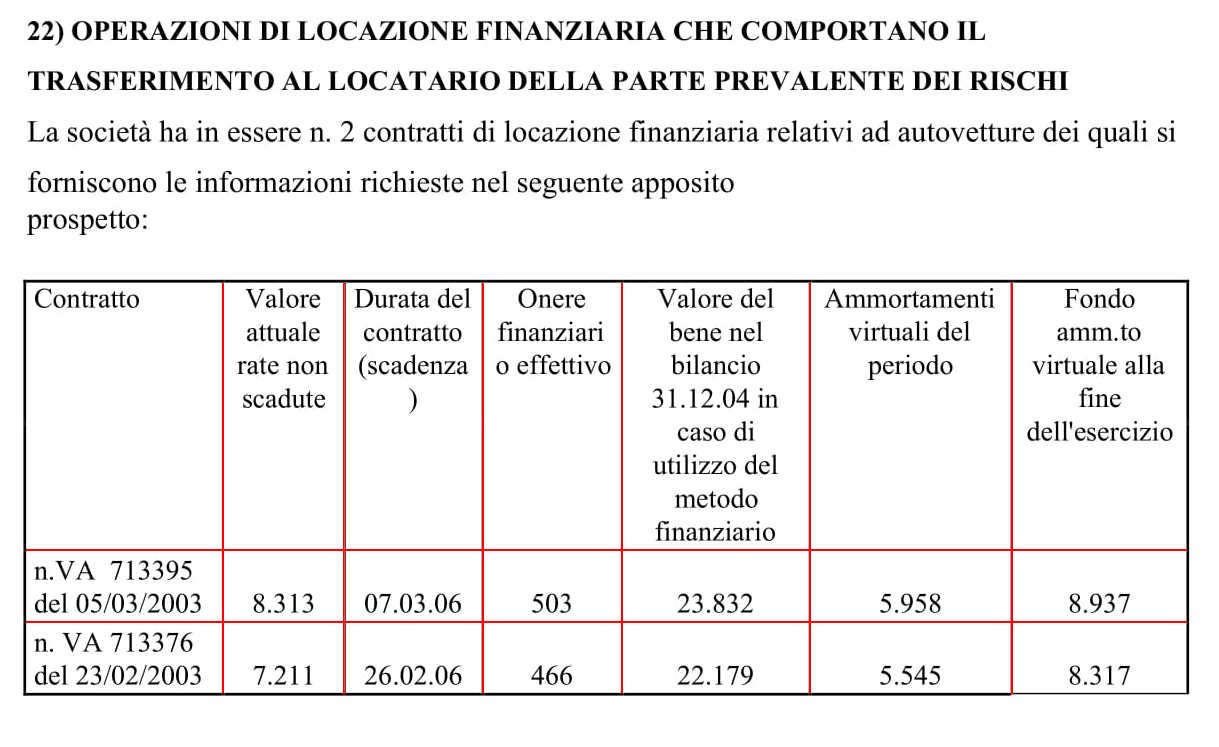
\includegraphics[width=\linewidth,height=40mm]{img/implementation/textlineEmpty.png}
\caption{Empty lines} \label{fig:1b}
\end{subfigure}
\qquad
\begin{subfigure}{0.45\textwidth}
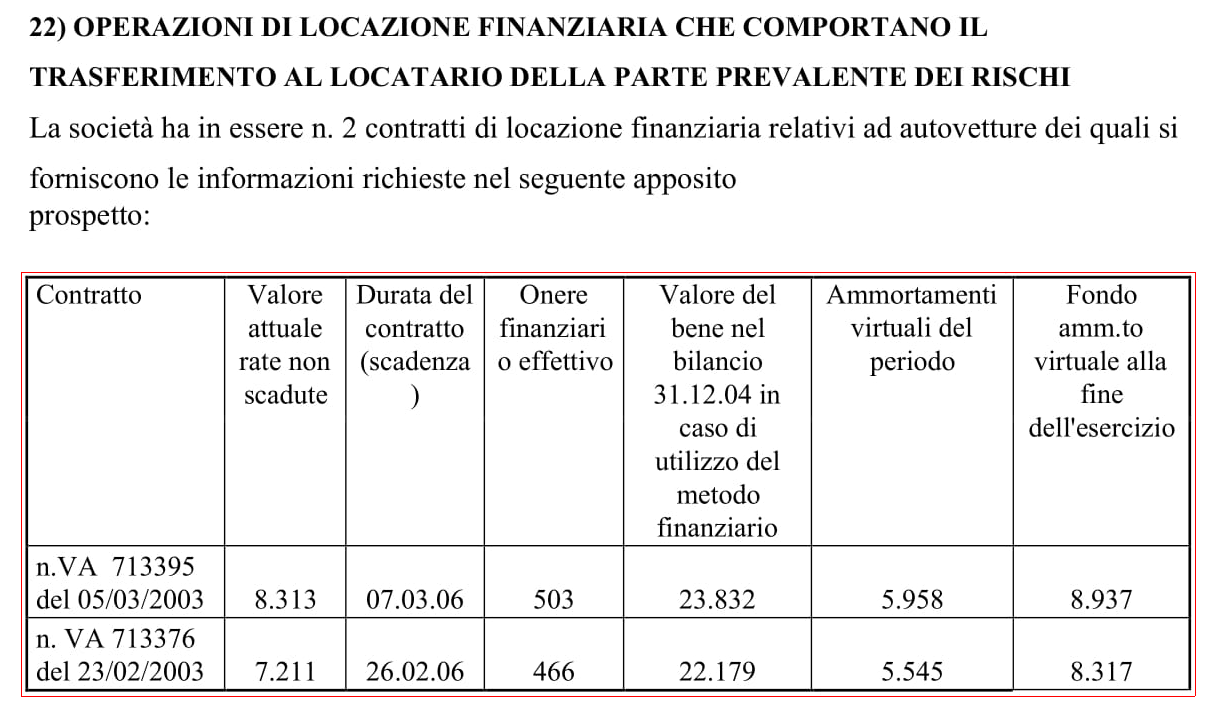
\includegraphics[width=\linewidth,height=40mm]{img/implementation/textlineTable.png}
\caption{Table textline} \label{fig:1c}
\end{subfigure}
\caption{Deletion of unnecessary lines} \label{fig:1}
\end{figure}

Once this step of the algorithm is done, we are left only with lines that contain symbols and can be a part of the table.

\item[Column detection]
Upon obtaining the textlines, we try to determine the all their their columns from the symbols they contain. This is done for each line individually. Firstly, we merge symbols into words. After that, we merge words into columns. Although we could simply just merge symbols into columns and ignore the whole processing of the words, this would leave us with no spaces between words in individual columns.

We start this process by getting all the spaces between individual symbols and sorting them by size. For a human eye, upon seeing this list, to determine the whitespace between individual words and columns is mostly a pretty easy task. Following are three lists of spaces and a visualized merge of our algorithm according to them:

\texttt{}{
1 1 2 2 2 3 3 3 3 3 3 3 3 3 3 3 3 4 4 4 4 5 15 15 16 16 18 18 227 235;

2 2 2 2 2 2 2 2 2 3 3 3 3 3 3 3 3 3 3 3 3 4 4 4 4 4 4 4 5 5 6 15 15 16 17 165 235;

1 1 1 2 2 2 3 3 3 3 3 3 3 3 3 3 3 4 4 4 4 4 4 4 4 5 5 15 15 15 17 17 17 18 134 235;}

\begin{figure}[H]
\hspace*{\fill} % separation between the subfigures
\begin{subfigure}{0.80\textwidth}
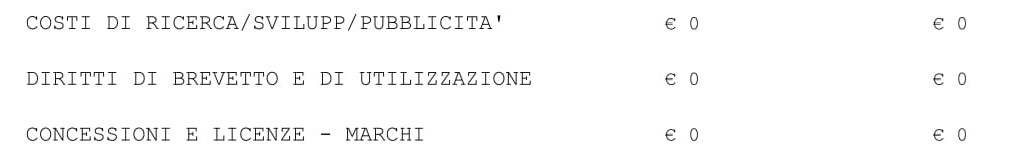
\includegraphics[width=\linewidth]{img/implementation/mergedOrig.jpg}
\caption{The original image} \label{fig:1b}
\end{subfigure}
\begin{subfigure}{0.80\textwidth}
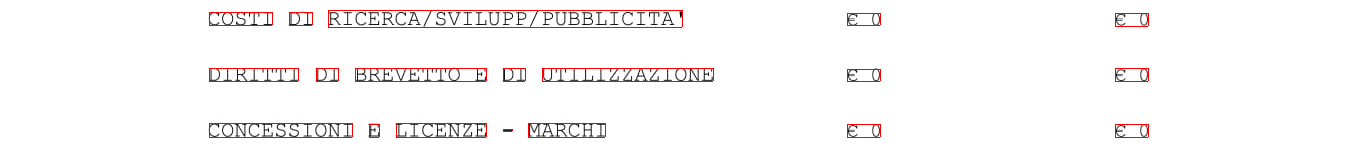
\includegraphics[width=\linewidth]{img/implementation/mergedWords.png}
\caption{Merged into words} \label{fig:1c}
\end{subfigure}
\hspace*{\fill} % separation between the subfigures
\begin{subfigure}{0.80\textwidth}
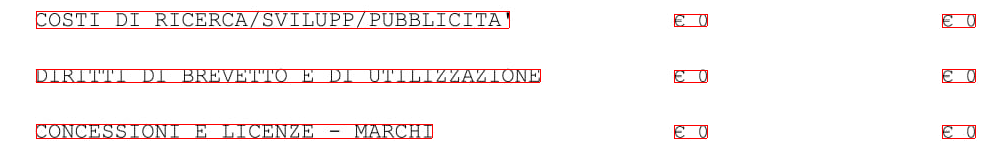
\includegraphics[width=\linewidth]{img/implementation/mergedCols.png}
\caption{Merged into columns} \label{fig:1c}
\end{subfigure}
\caption{The process of merging symbols of a textline} \label{fig:1}
\end{figure}

\xxx{opat netusim ako formatovat, ma ten obrazok byt vobec tu?}

It is quite obvious that the word whitespace will therefore be around 5-6 in all cases and column whitespace 227, 165 and 134 respectively. In our program, we determined these whitespaces by iterating over all the spaces. Once we find two subsequent spaces that have "great difference between their values", we assume the greater one to be the whitespace of either words, columns or both.

So how do we determine whether the difference is too great? For both word and column whitespaces, we calculate a so-called \emph{multiplicator factor} and use it according to\xxx{like?} the next code snippet that is used for the determination of the word whitespace.

\begin{code}
for (it; it != all_spaces.end() - 1; it++)
{
	// get multiplication factor of current space
	double multi_factor = get_multi_factor_words(*it, constant);
	if (*std::next(it) >= multi_factor * *it)
	{
		// found the word whitespace at *std::next(it)
		// code to execute once the whitespace is found
	}
}
\end{code}

The simplest observation is --- the greater the current space is, the less the multiplication factor should be. Based on this, many different values and curves have been tried for the determination of multiplication factor. First observations from these attempts led to the estimation that the best curve to use would be logarithmic. However, the current implementation seemed to worked well enough and was therefore left as it is.

The determination of the column whitespace was done similarly. Although the function determining the multiplication factor was altered, the idea stayed the same.

Upon determining the column and word whitespaces, the only thing left is to merge symbols by these whitespaces.

The determination of whitespaces was probably the hardest part of the algorithm. There have been multiple different ideas for the implementation. The one that has been preferred most of the time was the idea of separating textlines according to their \emph{fonts} \xxx{tj. (aka, ako to napisem?) their heights}. The ones with similar fonts were assigned to same \emph{font category}, and the whitespace was then determined from the whole category. The word whitespace recognition worked slightly better with this approach. However, the determination of columns had a higher chance of failure, as the sizes of column spaces differed greatly and the algorithm had a problem with finding the point where word spaces end and column spaces start. Therefore, this simpler approach was chosen.

Another approach was to simply determine the size of the column space by a constant, e.g. word\_whitespace*constant = column\_whitespace. Suprisingly, the results of this approach were comparable to those of the current implementation. However, it was deemed to fail when it came to small fonts or full-page tables, and had no room for improvement in contrast with the current approach.

\item[Table creation]

Once we have the information about columns for each textline, we can start searching for tables. The table detection algorithm is done by a simple $O(n)$ algorithm --- iterating the textlines from top to bottom and merging two consecutive textlines together if they belong to the same table.

Following is an algorithm used to determine whether two lines represented by columns are in the same table:

\xxx{To Do - sformatovat? :( }

\begin{algorithm}[H]
\caption{Are textlines in same table}
\begin{algorithmic}[1]
\State $iter\_first$ represents the current place we are when iterating over columns of first line
\State $iter\_second$ represents the current place we are when iterating over columns of second line
\While{true}
\If {either $iter\_first$ or $iter\_second$ is at the end of their line}
\If {at least one pair of columns was found that should be merged}
\State \emph{merge()}
\EndIf
\EndIf
\If {current\_columns\_overlap() } \Comment{a function that checks whether the bounding boxes of the two columns overlap in the x axis}
\If {found columns do not overlap with other existing columns in the x axis}
\State save the position of overlapping columns for future mergeing
\EndIf
\Else 
\State increase either $iter\_first$ or $iter\_second$ depending on which is poiting to the box that has a lower x-axis
\State continue
\EndIf
\State $iter\_first \gets iter\_first+1$
\State $iter\_second \gets iter\_second+1$
\EndWhile
\end{algorithmic}
\end{algorithm}

Merge of the textlines is done by merging columns that have been detected to overlap, and adding other columns with no such attribute. In a typical n*m table, every column should overlap with the one underneath it, which is also mostly the case when running this algorithm.

Once we have at least two merged textlines, we use this new merged line as a current textline. Therefore, when creating a table, we append new lines to the already merged ones. At the end of this algorithm, our current table is therefore represented as a textline with the information about its columns (and a list of textlines that are in the current table).

\item[Output creation]

What we care about when creating an output are table cells. We create these by simply overlaying \xxx{dobre slovo? prelozit} rows and columns and saving their common areas as cells. The problem arises with the existence of multi-line rows, that is, rows that often span over multiple Tesseract recognized textlines. In our implementation, a simple constant-based algorithm is added to recognize at least some of them and therefore merge multiple textlines into one row. The algorithm for this could be improved differently, which will be discussed in the next chapter. 

Once we obtain cells, the only thing left is to create a user-friendly representation of the recognized data. Here, the user has two options according to the parameter he sets in the command line environment. 

The first option is a simple image output. Recognized cells are therefore bordered \xxx{dobre slovo?} by colored boxes in the original input image and saved in a PNG file.

The other option is a json structure of the recognized cells, which also contains text within each cell. The json has the following structure:

\lstset{
    string=[s]{"}{"},
    stringstyle=\color{blue},
    comment=[l]{:},
    commentstyle=\color{black},
}
\begin{lstlisting}
{"all_tables": {
  "cols": number of columns,
  "rows": number of rows,
  "table_repres": {
    "h": height of table,
    "w": width of table,
    "x": the x-coordinate where the table starts
    "y": the y-coordinate where the table starts
  }
  "cells": [
        {
        "box": {
           "h": height of current cell,
           "w": width of current cell,
           "x": the x-coordinate where the cell starts,
           "y": they y-coordinate where the cells starts,
        },
        "cols_no": in which column of the table the cell is,
        "rows_no": in which row of the table the cell is,
        "text": the UTF8 text displayed in the cell
        },
        ...
        other cells
    ]
  }
  ...
  other tables
}
\end{lstlisting}


By default, both output options are selected and therefore two files are saved in the newly created \emph{results} directory inside the build directory.

\end{description}

\begin{figure}[H]
\begin{subfigure}{0.45\textwidth}
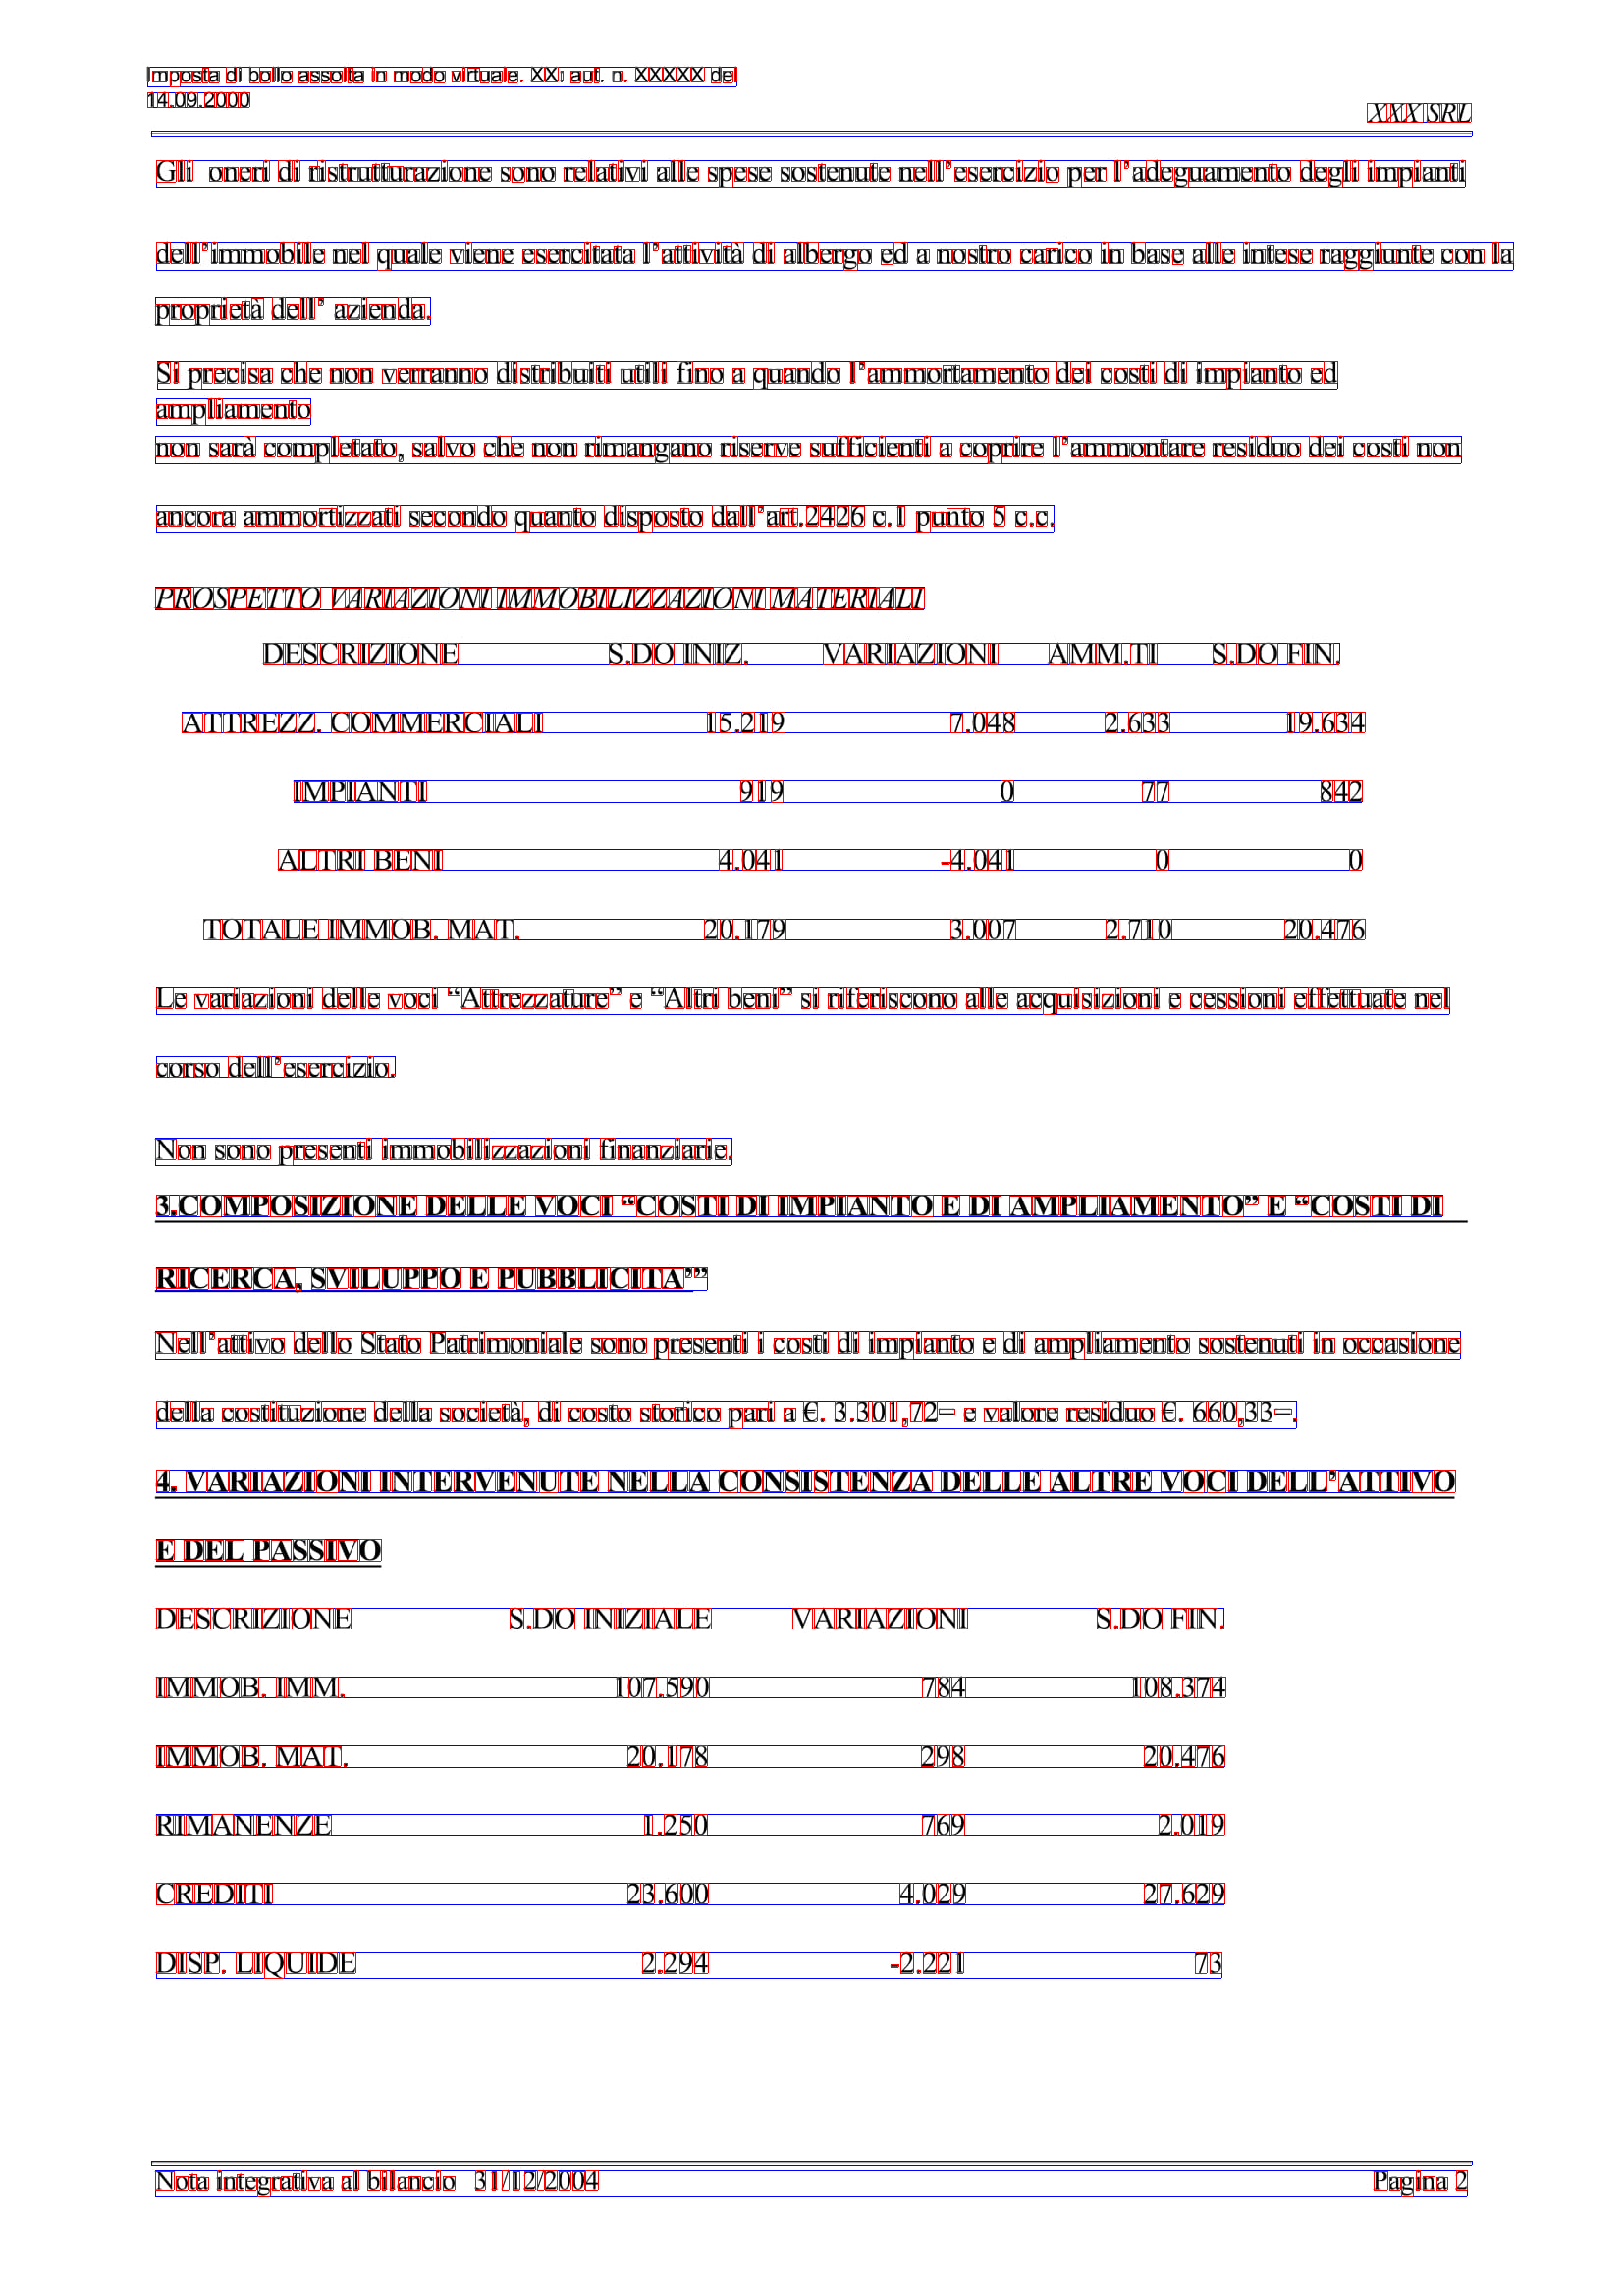
\includegraphics[width=\linewidth]{img/implementation/implem1.png}
\caption{Individual textlines (blue) and their symbols (red)} \label{fig:1b}
\end{subfigure}
\hspace*{\fill} % separation between the subfigures
\begin{subfigure}{0.45\textwidth}
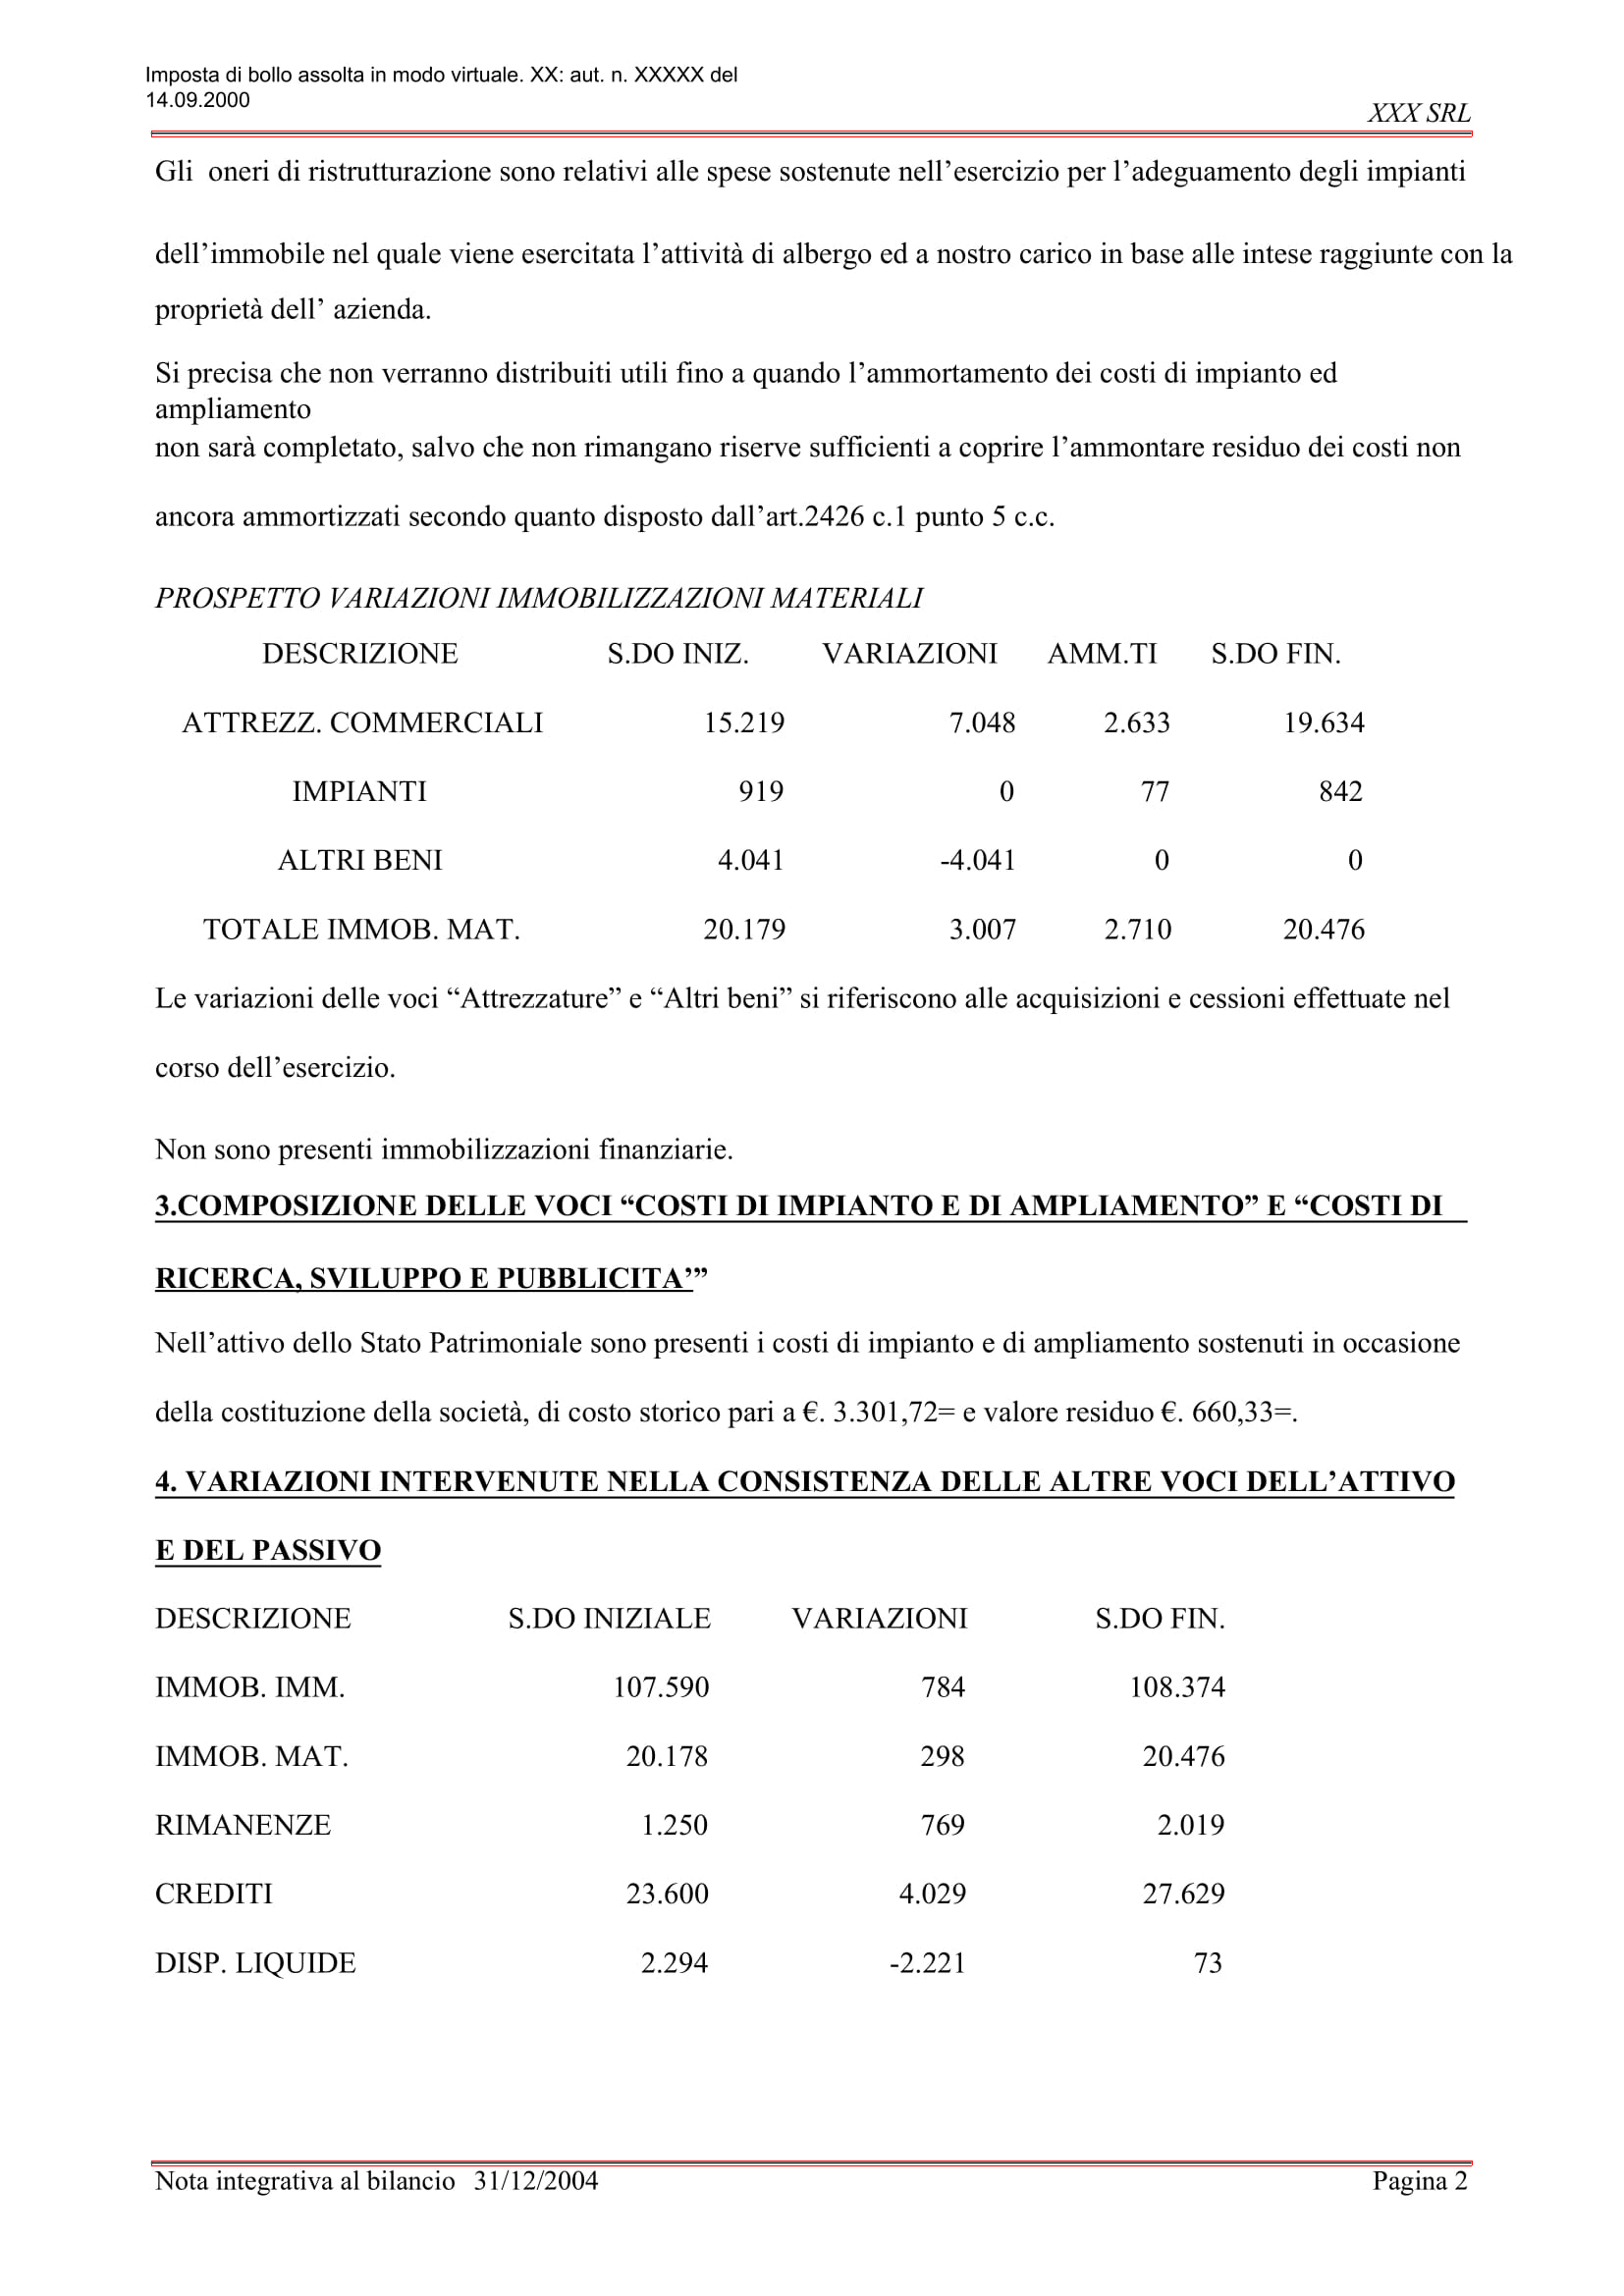
\includegraphics[width=\linewidth]{img/implementation/implem2.png}
\caption{Unnecessary lines} \label{fig:1b}
\end{subfigure}
\begin{subfigure}{0.45\textwidth}
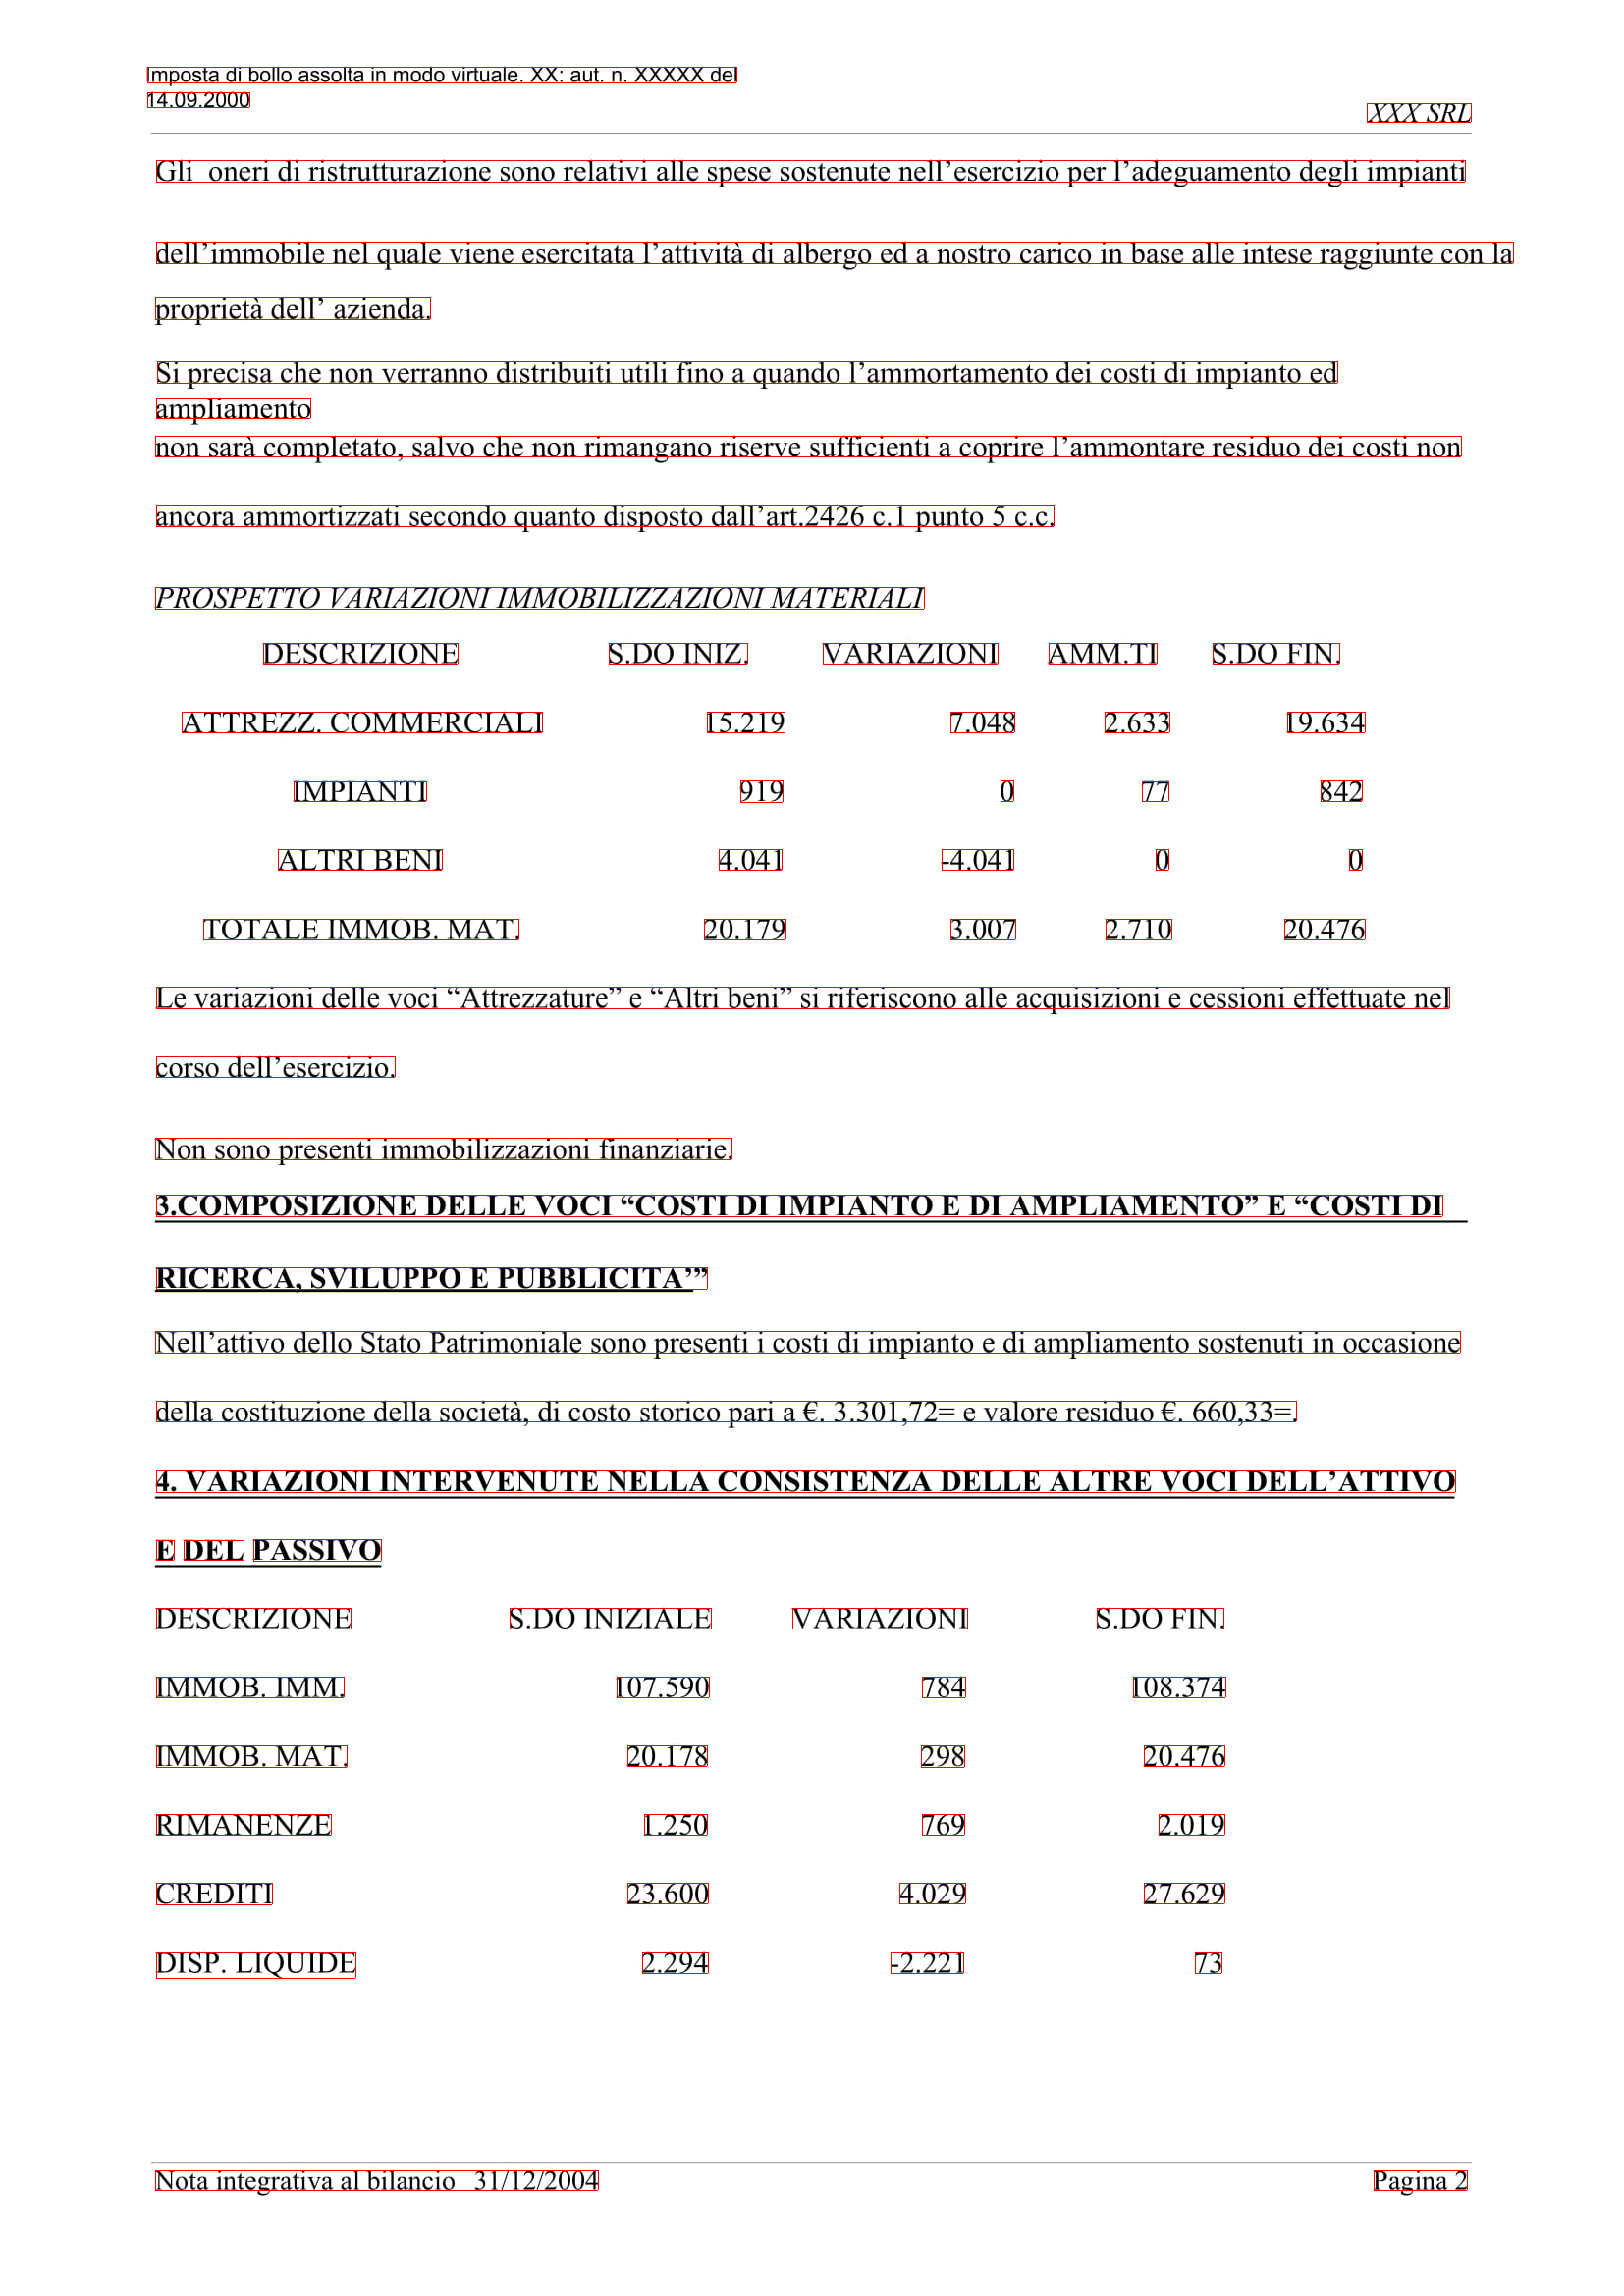
\includegraphics[width=\linewidth]{img/implementation/implem3.png}
\caption{Textlines merged into columns} \label{fig:1c}
\end{subfigure}
\hspace*{\fill} % separation between the subfigures
\begin{subfigure}{0.45\textwidth}
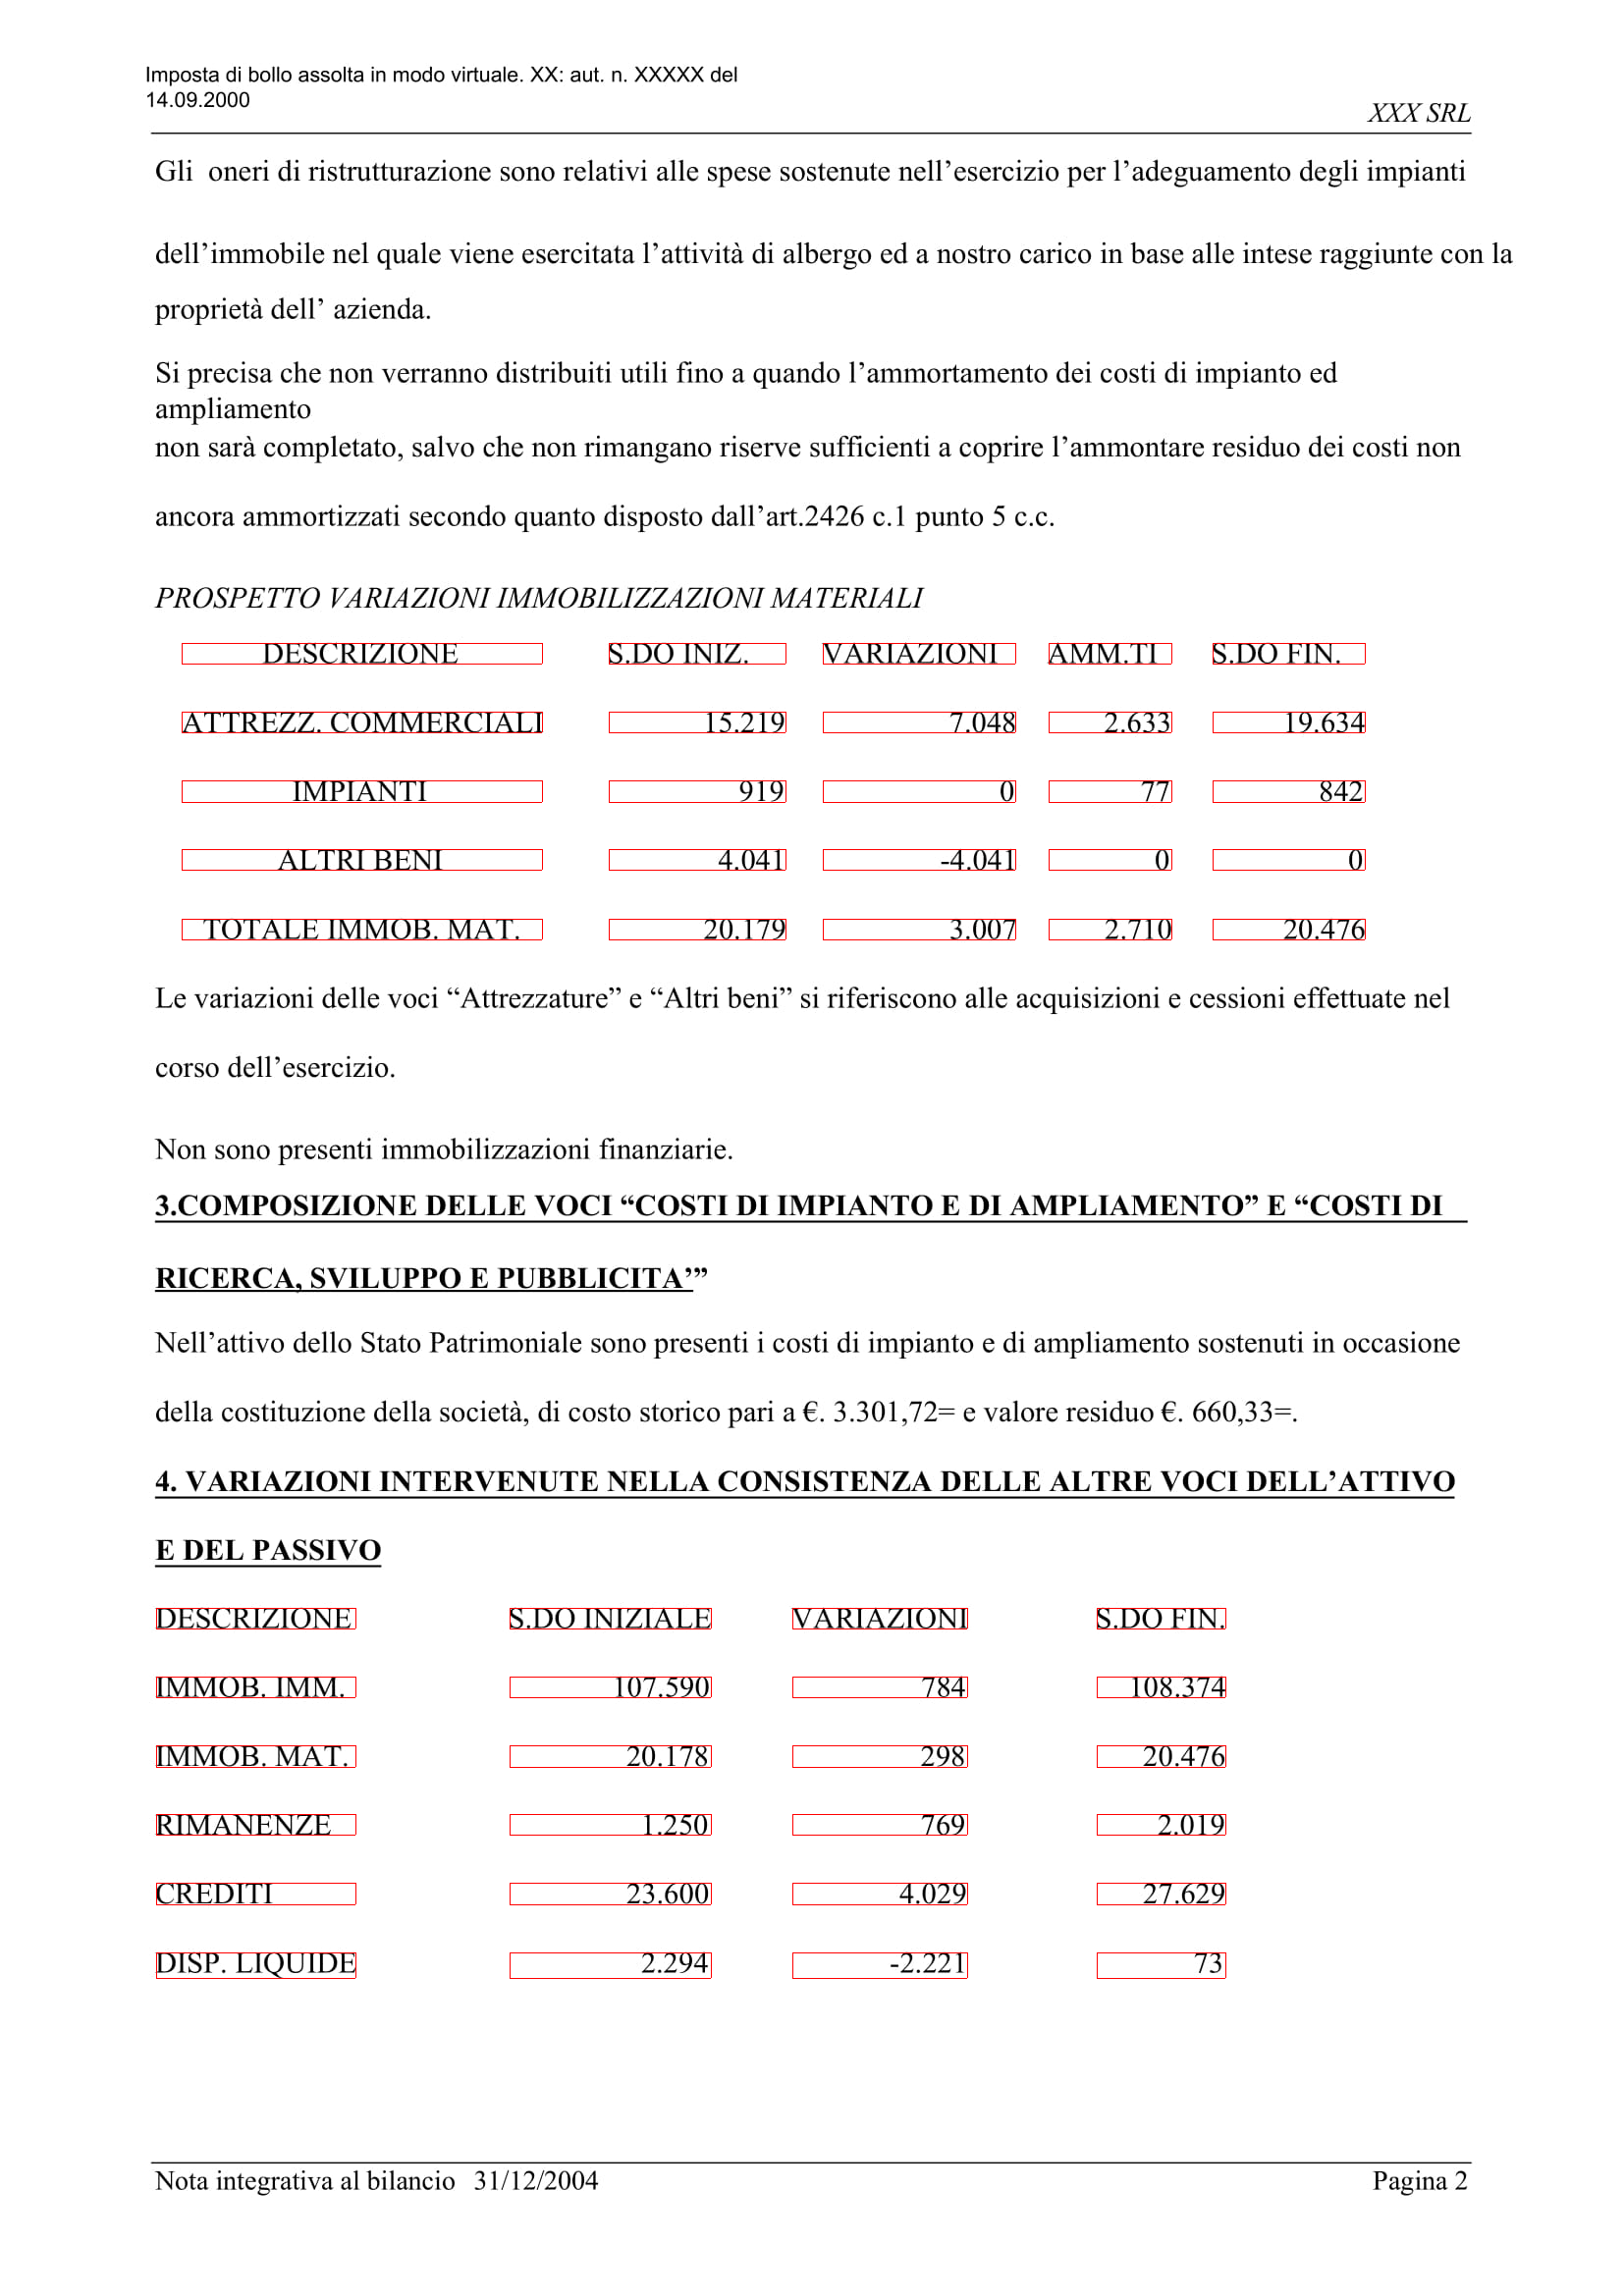
\includegraphics[width=\linewidth]{img/implementation/implem4.png}
\caption{The resulting cells} \label{fig:1c}
\end{subfigure}
\caption{The process of table recognition} \label{fig:1}
\end{figure}

\begin{figure}
    \noindent
	\makebox[\textwidth]{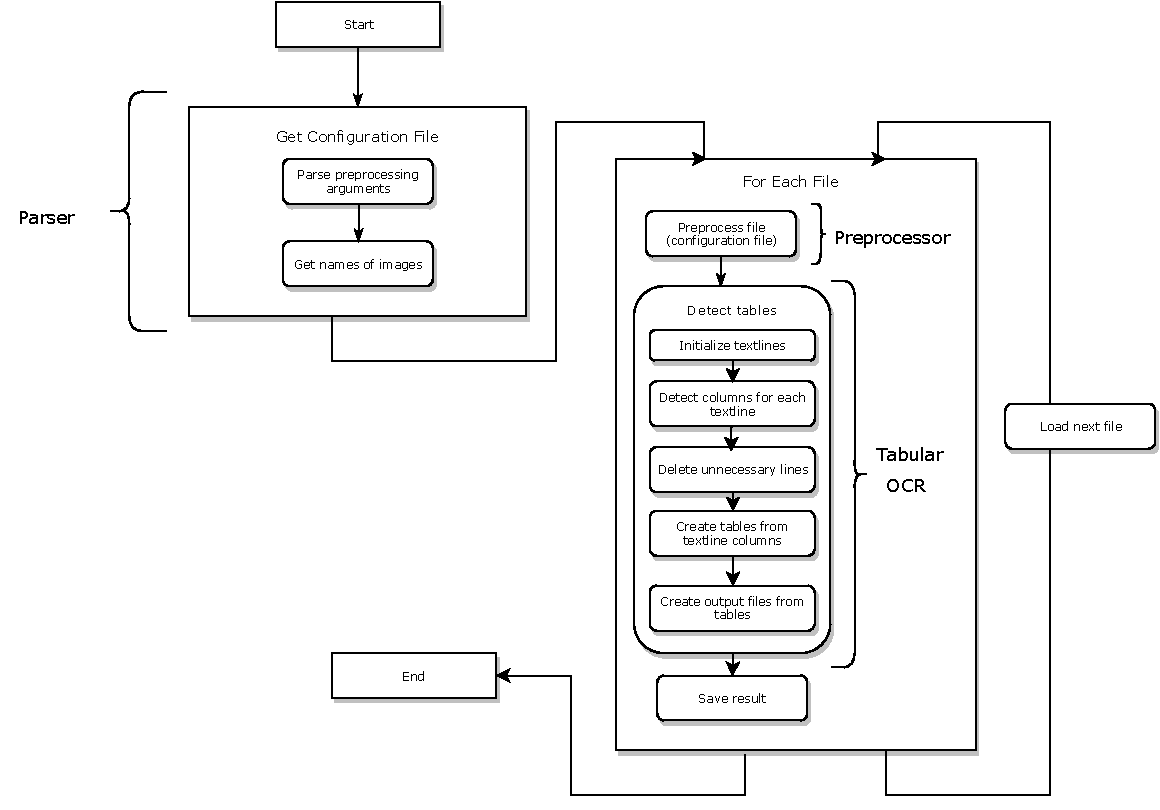
\includegraphics[width=\paperwidth-100pt]{../img/implementation/programFlow.pdf}}
	\caption{Program Flow Diagram}
	\label{fig:mff}
\end{figure}
